\subsection*{1}
    %Build a noninverting amplifier circuit as shown below. Use R1 = 100  and R2 = 10 k 
    %so that the amplifier gain is about 100.



    \begin{figure}[h!]
        \centering
        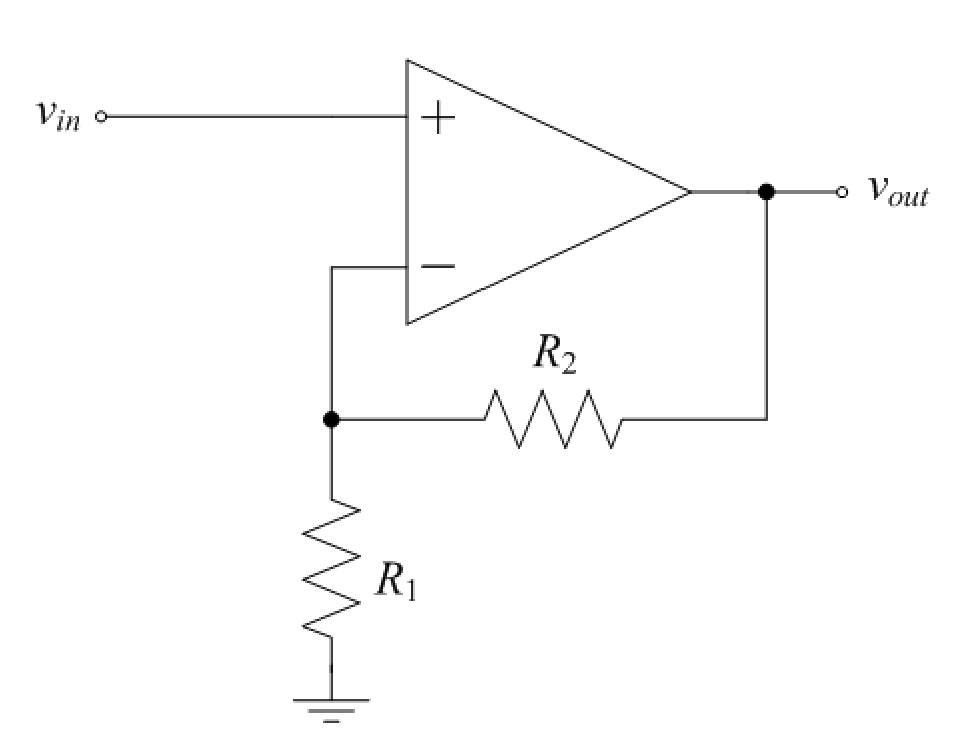
\includegraphics[width=6cm]{task2_1.png}
        \captionof{figure}{}
    \end{figure}

\subsection*{2}
    %Using  a  Bode  Analyzer  measure  the  AC  characteristics  of  the  circuit in  the  frequency
    %range 100 Hz to 50 kHz. Use 10 steps per decade and input signal amplitude of 20 mV.
    %Find the gain-bandwidth product (GBW) of the operational amplifier and compare it to
    %the nominal value (1 MHz). 


\subsection*{3}
    %Build a voltage follower circuit as shown below:

    \begin{figure}[h!]
        \centering
        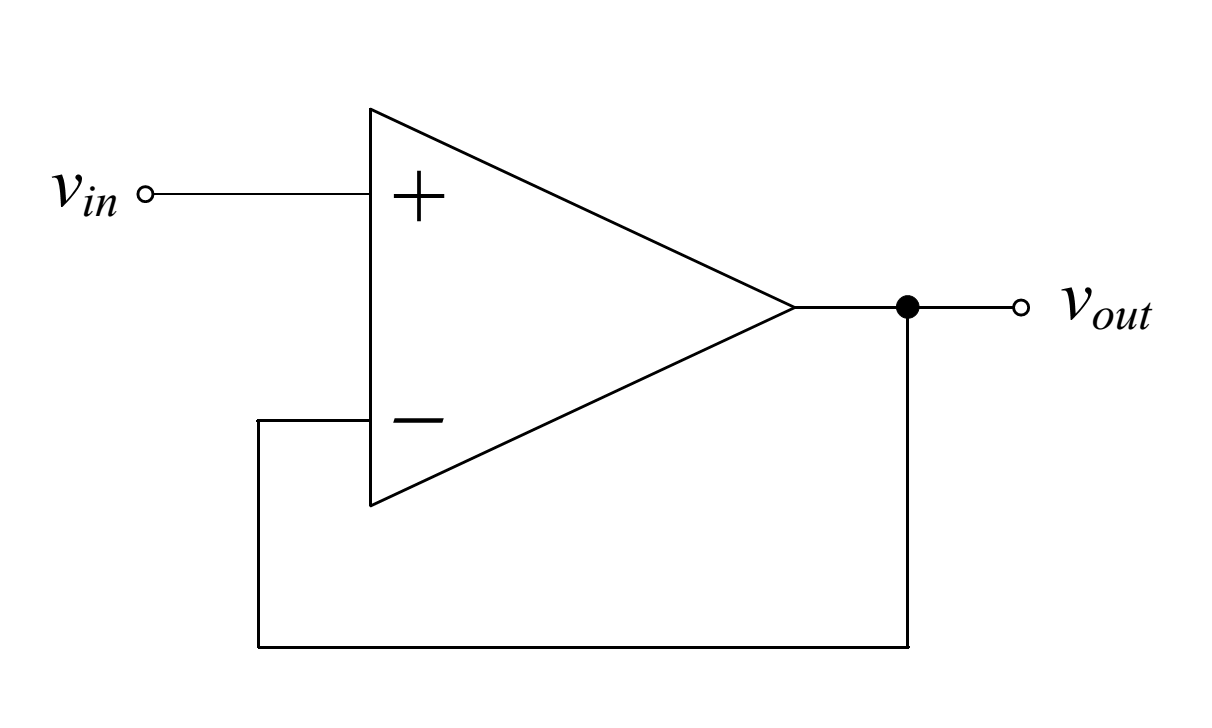
\includegraphics[width=6cm]{task2_3.png}
        \captionof{figure}{}
    \end{figure}


\subsection*{4}
    %Apply  a  rectangular  waveform  (amplitude  around  2.5 V)  to  the  input  of  the  circuit  and
    %observe both the input and the output signal using the oscilloscope. Determine the slew- 
    %rate (SR) of the operational amplifier and compare it to the nominal value (0.5 V/µs).